\documentclass[main.tex]{subfiles}

\begin{document}
\chapter{Phonon mediated tunneling into \TaS (BETTER TITLE NEEDED)}\label{ch:sts_gap_tas2}

%\section{Scanning Tunneling Spectroscopy}

\acrfull{sts} is an experimental technique in which a \acrfull{stm} is used to map the density of states of a material.

\todo{introduction stm/sts}

Stipe et al. noted that the tunneling current in \acrshort{sts} can also identify phonon modes of the material measured \cite{stipe_single-molecule_1998} (vibrational modes of a single molecule in this case).
Similarly, a gap feature around the fermi level in the measured DOS on graphene \cite{zhang_giant_2008} was explained with electron-phonon interaction \cite{wehling_phonon-mediated_2008}.

The underlying mechanism is that electrons can elastically tunnel into graphene at the Fermi level near the \(\vb{K}\) point. \todo{Graphic for that would be nice}
This elastic process is suppressed because the wave function at the initial state i.e. the wave functions at the tip have a momentum distribution centered at \(\vb*{k}_{\parallel} = 0\), so the tunneling matrix element is suppressed for large \(\vb*{k}\) \cite{vitali_phonon_2004}.
For electron energies larger than the energy 

In a 2019 paper by Hall et al. \cite{hall_environmental_2019}, a similar gap feature with a width of \(2 \Delta = \SI[separate-uncertainty = true]{32 \pm 9}{\milli\eV}\) was recorded in an \acrshort{sts} measurement on \TaS.


\begin{figure}
    \centering
    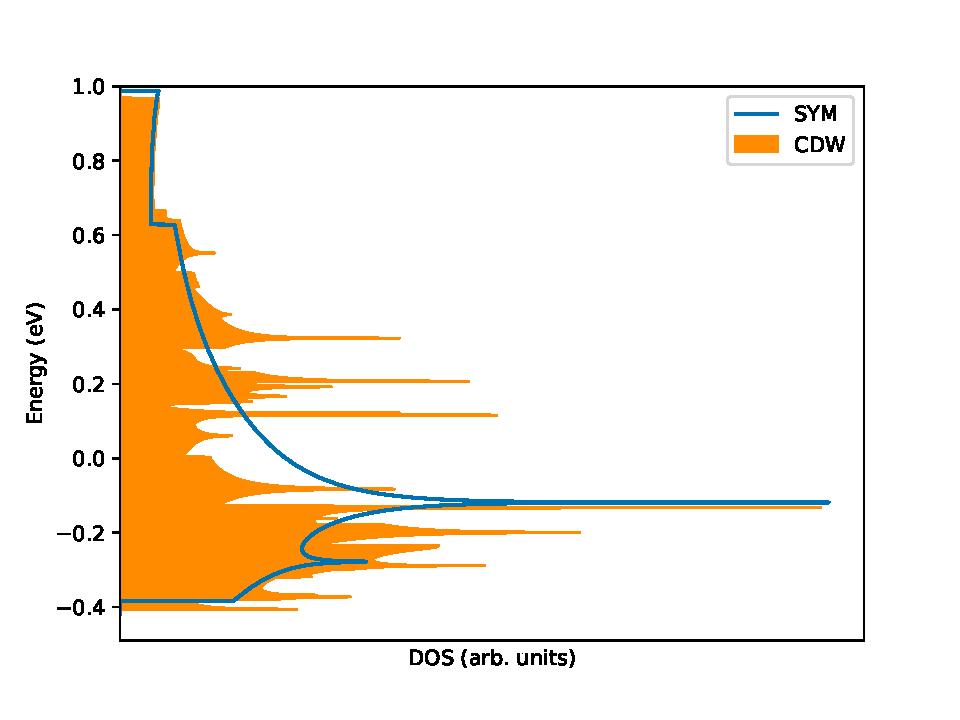
\includegraphics[width=0.6\textwidth]{tas2_dos.pdf}
    \caption{Density of states}
\end{figure}


\end{document}